\documentclass[11pt,a4paper,english,twocolumn]{article}
%\usepackage[T1]{fontenc}
\usepackage[utf8]{inputenc}
\usepackage{babel}
\usepackage{blindtext}
\usepackage{hyperref}
\usepackage{graphicx}
%\usepackage{wrapfig}

\title{\textbf{Slovene NLTK Tagger}}
\author{
Niko Colnerič \\
\footnotesize Faculty of Computer and \\
\footnotesize Information Science \\
\footnotesize University of Ljubljana \\
\and
Nejc Banič \\
\footnotesize Faculty of Computer and \\
\footnotesize Information Science \\
\footnotesize University of Ljubljana \\
}

\begin{document}
\maketitle
\thispagestyle{empty}
%\pagebreak

\section*{Abstract - NIKICC}
This paper describes the process of building Slovene tagger for use in NLTK.  
\section{Introduction - NIKICC}
Tagger processes a sequence of words and attaches a part of speech tag to each word. We implemented tagger for Slovene language in NLTK. NLTK stands for Natural Language Toolkit and is a library for use in Python (currently for version below 3, we used 2.7). NLTK already has some taggers for English and some other languages. Our goal was to implement NLTK tagger for Slovene language. The result of this project depends on two other larger projects. First is \textit{JOS}\cite{JOS}(in Slovene it stands for: "Jezikoslovno Označevanje Slovenskega jezika"), from which we used the corpuses (large and structured set of texts). Second, \textit{nltk-trainer}\cite{nltk-trainer}, is an open-source project hosting on Github, which was used for actual training of the tagger on Slovene sentences. Our work based mainly on putting all this pieces together into a working Slovene NLTK tagger.
\section{JOS corpora}
The basic component for building Slovene tagger is \textbf{JOS corpora}. It contains collections of various text in Slovenian language with annotation. For our project we used jos1M corpus that contain 1 million words with it's appropriate lemmas and morphosyntactic descriptions. The JOS is compatible with Slovene\textit{ MULTEXT-East morphosyntactic specifications Version 4}\cite{MULTEXT-East}. It basic purpose is to define word classes. For each class there are various attributes and their appropriate values, which they can be mapped into morphosyntactic descriptions (i.e. MSD). The structure of JOS corpora is in  \textbf{Extensible Markup Language (XML)}. We can easily manipulate XML files in various programming languages (e.g. Python with xml.dom.minidom). This is mandatory because \textit{nltk-trainer}\cite{nltk-trainer} expects special form of input file. For further information see \ref{Corpus transformation}.
\section{Nltk-trainer - NIKICC}
Nltk-trainer\cite{nltk-trainer} is project, whose author is Jacob Perkins, from which we took the code for building the tagger. We almost exclusively used the script \textit{train\_tagger.py}, which has the ability to generate NLTK taggers. Its mandatory argument is corpus in .pos format. Other optional arguments can choose wheather to generate a Sequential Tagger, a Brill Tagger or a Classifier Based Tagger. It also has the possibility to set default tag (the tag for words, for which the tagger doesn't know how to tag) and wheather to evaluate the tagger or not. For evaluation of the tagger (section \ref{Evaluation}) this argument was used. 
\section{Taggers description}
\subsection{Trigram tagger}
\textit{TODO - NIKICC}
\subsection{Brill tagger}
\textit{TODO - BANIČ}
\subsection{Naive Bayes tagger}
\textit{TODO - BANIČ}
\section{Implementation}
\subsection{Corpus transformation}\label{Corpus transformation}
\textit{TODO - BANIČ}
\subsection{Training the tagger}
\textit{TODO - NIKICC}
\subsection{Usage with NLTK}
\textit{TODO - BANIČ}
\subsection{Encoding problems}
\textit{TODO - BANIČ}
\section{Evaluation}\label{Evaluation}
\textit{TODO - NIKICC}
Average accuracy BrillTagger 0.852931.
Average accuracy NaiveBayes 0.848985.
Average accuracy TrigramTagger 0.831711.

\begin{figure}[h]
\begin{center}
\leavevmode
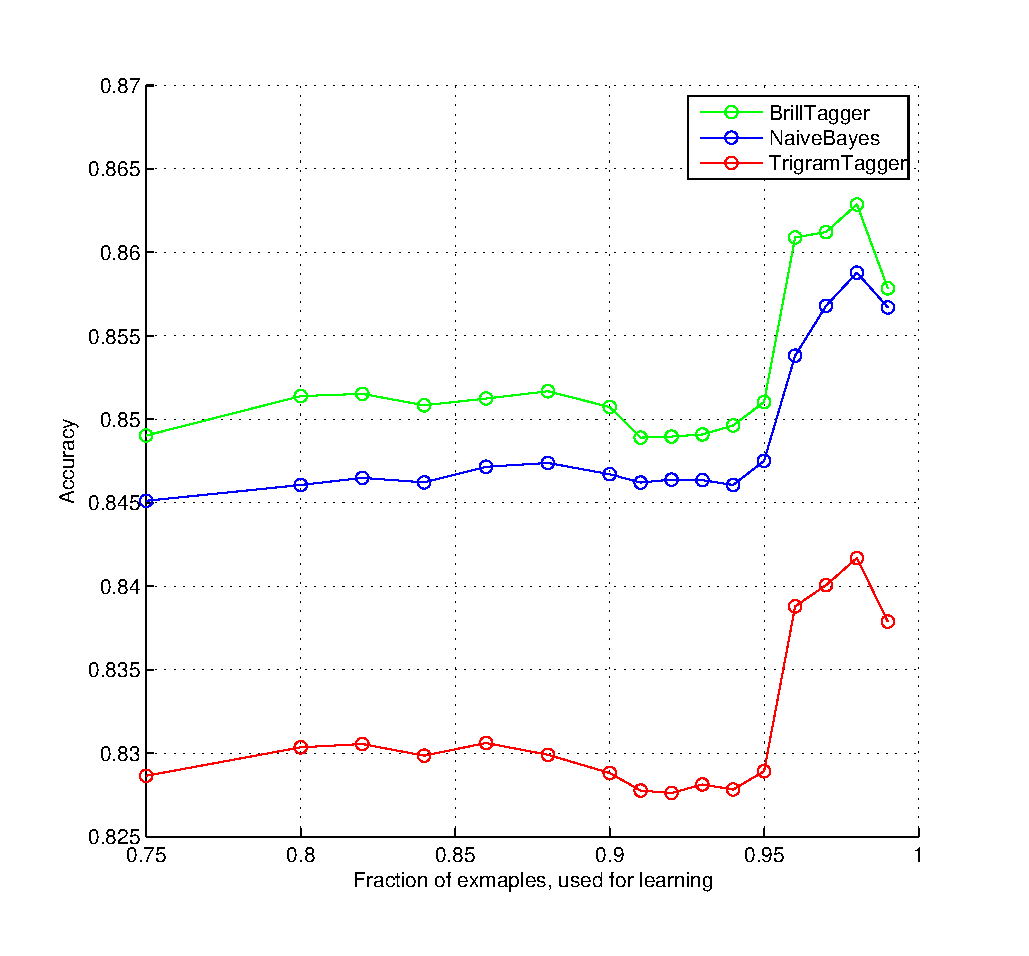
\includegraphics[width=0.6\textwidth]{../evaluation/graph.eps} 
\end{center}
\caption{Evaluation results, with different fractions}
\label{fig:evaluation}
\end{figure}

\section{Conclusion}
\textit{TODO - BANIČ}

%\thispagestyle{empty}
\begin{thebibliography}{99}
\bibitem{JOS} \url{http://nl.ijs.si/jos/}
\bibitem{nltk-trainer} \url{https://github.com/japerk/nltk-trainer}
\bibitem{MULTEXT-East} \url{http://nl.ijs.si/ME/V4/msd/html/msd-sl.html}
\end{thebibliography}
\end{document}
